% (find-LATEX "2023-1-C2-intro.tex")
% (defun c () (interactive) (find-LATEXsh "lualatex -record 2023-1-C2-intro.tex" :end))
% (defun C () (interactive) (find-LATEXsh "lualatex 2023-1-C2-intro.tex" "Success!!!"))
% (defun D () (interactive) (find-pdf-page      "~/LATEX/2023-1-C2-intro.pdf"))
% (defun d () (interactive) (find-pdftools-page "~/LATEX/2023-1-C2-intro.pdf"))
% (defun e () (interactive) (find-LATEX "2023-1-C2-intro.tex"))
% (defun o () (interactive) (find-LATEX "2022-2-C2-intro.tex"))
% (defun u () (interactive) (find-latex-upload-links "2023-1-C2-intro"))
% (defun v () (interactive) (find-2a '(e) '(d)))
% (defun d0 () (interactive) (find-ebuffer "2023-1-C2-intro.pdf"))
% (defun cv () (interactive) (C) (ee-kill-this-buffer) (v) (g))
%          (code-eec-LATEX "2023-1-C2-intro")
% (find-pdf-page   "~/LATEX/2023-1-C2-intro.pdf")
% (find-sh0 "cp -v  ~/LATEX/2023-1-C2-intro.pdf /tmp/")
% (find-sh0 "cp -v  ~/LATEX/2023-1-C2-intro.pdf /tmp/pen/")
%     (find-xournalpp "/tmp/2023-1-C2-intro.pdf")
%   file:///home/edrx/LATEX/2023-1-C2-intro.pdf
%               file:///tmp/2023-1-C2-intro.pdf
%           file:///tmp/pen/2023-1-C2-intro.pdf
%  http://anggtwu.net/LATEX/2023-1-C2-intro.pdf
% (find-LATEX "2019.mk")
% (find-Deps1-links "Caepro5 Piecewise1")
% (find-Deps1-cps   "Caepro5 Piecewise1")
% (find-Deps1-anggs "Caepro5 Piecewise1")
% (find-CN-aula-links "2023-1-C2-intro" "2" "c2m231intro" "c2in")
% (find-MM-aula-links "2023-1-C2-intro" "C2" "c2m231intro" "c2in")

% «.defs»			(to "defs")
% «.defs-caepro»		(to "defs-caepro")
% «.title»			(to "title")
% «.links»			(to "links")
% «.semicirculo»		(to "semicirculo")
% «.releia-a-dica-7»		(to "releia-a-dica-7")
% «.gramatica»			(to "gramatica")
% «.gramatica-fig»		(to "gramatica-fig")
% «.pessimas-noticias»		(to "pessimas-noticias")
% «.sempre-e-nunca»		(to "sempre-e-nunca")
% «.justificativas»		(to "justificativas")
% «.atirei»			(to "atirei")
% «.imagens-de-intervalos»	(to "imagens-de-intervalos")
% «.sobre-portugues»		(to "sobre-portugues")
% «.sobre-portugues-2»		(to "sobre-portugues-2")
% «.banana»			(to "banana")
% «.unexpected-eof»		(to "unexpected-eof")
% «.ana-leticia»		(to "ana-leticia")
% «.retas-reversas»		(to "retas-reversas")
% «.contexto»			(to "contexto")
%
% «.formulas-e-hipoteses»	(to "formulas-e-hipoteses")
% «.aulas-expositivas»		(to "aulas-expositivas")
% «.formal-vs-coloquial»	(to "formal-vs-coloquial")

% «.explicando-o-PDF»		(to "explicando-o-PDF")
% «.escreva-hipotese»		(to "escreva-hipotese")
% «.monitoria»			(to "monitoria")



% <videos>
% Video (not yet):
% (find-ssr-links     "c2m231intro" "2023-1-C2-intro")
% (code-eevvideo      "c2m231intro" "2023-1-C2-intro")
% (code-eevlinksvideo "c2m231intro" "2023-1-C2-intro")
% (find-c2m231introvideo "0:00")

\documentclass[oneside,12pt]{article}
\usepackage[colorlinks,citecolor=DarkRed,urlcolor=DarkRed]{hyperref} % (find-es "tex" "hyperref")
\usepackage{amsmath}
\usepackage{amsfonts}
\usepackage{amssymb}
\usepackage{pict2e}
\usepackage[x11names,svgnames]{xcolor} % (find-es "tex" "xcolor")
\usepackage{colorweb}                  % (find-es "tex" "colorweb")
%\usepackage{tikz}
%
% (find-dn6 "preamble6.lua" "preamble0")
%\usepackage{proof}   % For derivation trees ("%:" lines)
%\input diagxy        % For 2D diagrams ("%D" lines)
%\xyoption{curve}     % For the ".curve=" feature in 2D diagrams
%
\usepackage{edrx21}               % (find-LATEX "edrx21.sty")
\input edrxaccents.tex            % (find-LATEX "edrxaccents.tex")
\input edrx21chars.tex            % (find-LATEX "edrx21chars.tex")
\input edrxheadfoot.tex           % (find-LATEX "edrxheadfoot.tex")
\input edrxgac2.tex               % (find-LATEX "edrxgac2.tex")
%\usepackage{emaxima}              % (find-LATEX "emaxima.sty")
%
% (find-es "tex" "geometry")
\usepackage[a6paper, landscape,
            top=1.5cm, bottom=.25cm, left=1cm, right=1cm, includefoot
           ]{geometry}
%
\begin{document}

% \catcode`\^^J=10
% \directlua{dofile "dednat6load.lua"}  % (find-LATEX "dednat6load.lua")
% %L dofile "Piecewise1.lua"           -- (find-LATEX "Piecewise1.lua")
% %L dofile "QVis1.lua"                -- (find-LATEX "QVis1.lua")
% %L dofile "Pict3D1.lua"              -- (find-LATEX "Pict3D1.lua")
% %L dofile "C2Formulas1.lua"          -- (find-LATEX "C2Formulas1.lua")
% %L Pict2e.__index.suffix = "%"
% \pu
% \def\pictgridstyle{\color{GrayPale}\linethickness{0.3pt}}
% \def\pictaxesstyle{\linethickness{0.5pt}}
% \def\pictnaxesstyle{\color{GrayPale}\linethickness{0.5pt}}
% \celllower=2.5pt

% «defs»  (to ".defs")
% (find-LATEX "edrx21defs.tex" "colors")
% (find-LATEX "edrx21.sty")

\def\u#1{\par{\footnotesize \url{#1}}}

\def\drafturl{http://anggtwu.net/LATEX/2023-1-C2.pdf}
\def\drafturl{http://anggtwu.net/2023.1-C2.html}
\def\draftfooter{\tiny \href{\drafturl}{\jobname{}} \ColorBrown{\shorttoday{} \hours}}

\def\asf#1{〈\textsf{#1}〉}
\def\Expr{\asf{expr}}
\def\Just{\quad\asf{justificativa}}

\catcode`\^^J=10
\directlua{dofile "dednat6load.lua"}  % (find-LATEX "dednat6load.lua")

% «defs-caepro»  (to ".defs-caepro")
%L dofile "Caepro5.lua"              -- (find-angg "LUA/Caepro5.lua" "LaTeX")
\def\Caurl   #1{\expr{Caurl("#1")}}
\def\Cahref#1#2{\href{\Caurl{#1}}{#2}}
\def\Ca      #1{\Cahref{#1}{#1}}
\pu




%  _____ _ _   _                               
% |_   _(_) |_| | ___   _ __   __ _  __ _  ___ 
%   | | | | __| |/ _ \ | '_ \ / _` |/ _` |/ _ \
%   | | | | |_| |  __/ | |_) | (_| | (_| |  __/
%   |_| |_|\__|_|\___| | .__/ \__,_|\__, |\___|
%                      |_|          |___/      
%
% «title»  (to ".title")
% (c2m231introp 1 "title")
% (c2m231introa   "title")

\thispagestyle{empty}

\begin{center}

\vspace*{1.2cm}

{\bf \Large Cálculo 2 - 2023.1}

\bsk

Aula 0: Introdução ao curso

e algumas dicas de estudo

\bsk

Eduardo Ochs - RCN/PURO/UFF

\url{http://anggtwu.net/2023.1-C2.html}

\end{center}

\newpage

% «links»  (to ".links")
% (c2m231introp 2 "links")
% (c2m231introa   "links")

% (mc2)

% Contas, computador, sintaxe, erros pequenos de conta
% (saptp 1 "title")
% (sapta   "title")
% (find-TH "2021aulas-por-telegram" "legendas")


% (find-LATEXfile "2022-C2-projeto-de-monitoria.tex" "Caracterização")



% livros diferentes usam linguagens diferentes: notação de Leibniz
% (c3m222p2p 6 "questao-2-gab")
% (c3m222p2a   "questao-2-gab")

% definicao: em integrais improprias a gente vai redefinir integral

% erro de sintaxe - gramática
% os computadores 


\newpage

%  ____        _       _ 
% | __ )  ___ | |__   / |
% |  _ \ / _ \| '_ \  | |
% | |_) | (_) | |_) | | |
% |____/ \___/|_.__/  |_|
%                        
% «semicirculo»  (to ".semicirculo")
% (c2m231introp 2 "semicirculo")
% (c2m231introa   "semicirculo")

{\bf Pedaço de semicírculo: seja como o Bob}


\scalebox{0.6}{\def\colwidth{9cm}\firstcol{

Imagina que você está numa turma de Cálculo 2 que tem dois ``Alex''es
-- vou chamar eles de Alex 1 e Alex 2 -- e um Bob. Numa das provas
dessa turma cai uma questão assim, sobre uma fórmula que calcula a
área de um pedaço de um semicírculo:

\begin{quote}

Calcule:
$$\intx{\sqrt{1-x^2}}$$

\end{quote}

Tanto o Alex 1 quanto o Alex 2 respondem essa questão dizendo só isso
aqui,
%
$$\frac12 \left( \arcsen(x) + x\sqrt{1-x^2} \right)
$$

e o Bob entrega uma resposta que tem uma página inteira de contas. Aí
na vista de prova o Bob está feliz porque ganhou todos os pontos dessa
questão e tanto o Alex 1 quanto o Alex 2 estão putíssimos porque
ganharam 0, e porque não conseguiram me convencer a aumentar as notas
deles.

}\anothercol{

O argumento do Alex 1 foi ``pô, professor, a resposta tá certa,
eu vi num livro e eu lembrava a fórmula, e eu até conferi ela no
computador depois'', o argumento do Alex 2 foi ``pô, professor, a
resposta tá certa, eu fiz as contas de cabeça e pensei tudo direito,
eu só não escrevi''...

\msk

\standout{Seja como o Bob!}

\bsk
\bsk
\bsk
\bsk
\bsk
\bsk

Porque é que os Alexes tiraram 0?

Que critério de correção eu usei aí?

Que critério de correção eu vou usar no curso?

Que nível de detalhe eu espero nas respostas?

\msk

Eu vou precisar de várias páginas pra responder tudo isso.

}}


\newpage

% «releia-a-dica-7»  (to ".releia-a-dica-7")
% (c2m231introp 3 "releia-a-dica-7")
% (c2m231introa   "releia-a-dica-7")
% (c2m212introp 3 "dica-7")
% (c2m212introa   "dica-7")

{\bf ``Releia a Dica 7''}

% A dica 7 é \ColorRed{INCRIVELMENTE} importante. Link:

\ssk

{\tiny

%              (find-TH "2021-1-C2-somas-1-dicas")
%  (find-angg "SUBTITLES/2021-1-C2-somas-1-dicas.lua")
% file:///home/edrx/TH/L/2021-1-C2-somas-1-dicas.html
\url{http://anggtwu.net/2021-1-C2-somas-1-dicas.html}

% (mpgp 5 "dicas")
% (mpg    "dicas")
% (c2m211somas1dp 7 "dica-7")
% (c2m211somas1da   "dica-7")
%    http://anggtwu.net/LATEX/material-para-GA.pdf#page=5
\url{http://anggtwu.net/LATEX/material-para-GA.pdf#page=5}

}

\scalebox{0.45}{\def\colwidth{12cm}\firstcol{

    1) Aprenda a testar tudo: contas, possíveis soluções de equações,
    representações gráficas de conjuntos...

    2) Cada ``seja'' ou ``sejam'' que aparece nestas folhas é uma
    definição, e você pode usá-los como exemplos de definições
    bem-escritas (ééé!!!!) pra aprender jeitos de escrever as suas
    definições.

    3) Em ``matematiquês'' a gente quase não usa termos como ``ele'',
    ``ela'', ``isso'', ``aquilo'' e ''lá'' --- ao invés disso a gente
    dá nomes curtos pros objetos ou usa expressões matemáticas pra
    eles cujo resultado é o objeto que a gente quer... mas {\sl quando
      a gente está discutindo problemas no papel ou no quadro} a gente
    pode ser referir a determinados objetos {\sl apontando pra eles
      com o dedo} e dizendo ``esse aqui''.

    4) Se você estiver em dúvida sobre o que um problema quer dizer
    tente escrever as suas várias hipóteses --- a prática de escrever
    as suas idéias é o que vai te permitir aos poucos conseguir
    resolver coisas de cabeça.

    5) Muitas coisas aparecem nestas folhas escritas primeiro de um
    jeito detalhado, e depois aos poucos de jeitos cada vez mais
    curtos. Você vai ter que aprender a completar os detalhes.

    6) Alguns exercícios destas folhas têm muitos subcasos. Nos
    primeiros subcasos você provavelmente vai precisar fazer as contas
    com todos os detalhes e verificá-las várias vezes pra não errar,
    depois você vai aprender a fazê-las cada vez mais rápido, depois
    vai poder fazê-las de cabeça, e depois você vai começar a
    visualizar o que as contas ``querem dizer'' e vai conseguir chegar
    ao resultado graficamente, sem contas; e se você estiver em dúvida
    se o seu ``método gráfico'' está certo você vai poder conferir se
    o ``método gráfico'' e o ``método contas'' dão aos mesmos
    resultados.

}\anothercol{

    7) Uma solução bem escrita pode incluir, além do resultado final,
    contas, definições, representações gráficas, explicações em
    português, testes, etc. Uma solução bem escrita é fácil de ler e
    fácil de verificar. Você pode testar se uma solução sua está bem
    escrita submetendo-a às seguinte pessoas: a) você mesmo logo
    depois de você escrevê-la --- releia-a e veja se ela está clara;
    b) você mesmo, horas depois ou no dia seguinte, quando você não
    lembrar mais do que você pensava quando você a escreveu; c) um
    colega que seja seu amigo; d) um colega que seja menos seu amigo
    que o outro; e) o monitor ou o professor. Se as outras pessoas
    acharem que ler a sua solução é um sofrimento, isso é mau sinal;
    se as outras pessoas acharem que a sua solução está claríssima e
    que elas devem estudar com você, isso é bom sinal. {\sl GA é um
      curso de escrita matemática:} se você estiver estudando e
    descobrir que uma solução sua pode ser reescrita de um jeito bem
    melhor, não hesite --- reescrever é um ótimo exercício.

}}





% Árvores
% (c2m222buracop 10 "exercicio-2")
% (c2m222buracoa    "exercicio-2")

% Cursos tradicionais
% (c2m212introp 2 "cursos-tradicionais")
% (c2m212introa   "cursos-tradicionais")

% Linguagem formal, gramática
% (c2m212introp 6 "sintaxe-2")
% (c2m212introa   "sintaxe-2")

% (c2m222buracop 5 "derivadas-formais")
% (c2m222buracoa   "derivadas-formais")


\newpage

%   ____                           _   _           
%  / ___|_ __ __ _ _ __ ___   __ _| |_(_) ___ __ _ 
% | |  _| '__/ _` | '_ ` _ \ / _` | __| |/ __/ _` |
% | |_| | | | (_| | | | | | | (_| | |_| | (_| (_| |
%  \____|_|  \__,_|_| |_| |_|\__,_|\__|_|\___\__,_|
%                                                  
% «gramatica»  (to ".gramatica")
% (c2m231introp 4 "gramatica")
% (c2m231introa   "gramatica")

{\bf Linguagem formal, gramática, sintaxe}


\scalebox{0.65}{\def\colwidth{13cm}\firstcol{

Veja se você consegue entender a figura da próxima página...

Eu peguei ela daqui, com pequenas adaptações:

\url{https://en.wikipedia.org/wiki/Context-free_grammar}

\msk

A parte à esquerda dela é a ``gramática'' de uma certa linguagem
formal, e a parte à direita dela mostra como uma certa expressão é
``parseada'' nessa linguagem formal.

\msk

Todas as linguagens de programação têm gramáticas bem definidas.
Quando a gente está trabalhando numa linguagem com uma gramática bem
definida é fácil definir quais expressões são válidas nela -- uma
expressão é válida quando ela é ``parseável'' -- e quais expressões
têm erros de sintaxe -- as que não são ``parseáveis''.

\msk

Em Prog 1 você aprendeu C, e você viu que o compilador podia rejeitar
os seus programas por vários motivos... por exemplo:

1. erros de sintaxe,

2. erros de tipo,

3. símbolos não declarados.

\msk

Se você quiser entender direito como compiladores detectam erros dos
tipos 2 e 3, dê uma olhada na página 99 do livro do Thain:

% (find-books "__comp/__comp.el" "thain")
% (find-books "__comp/__comp.el" "thain" "99")

\ssk

{\footnotesize

%    https://www3.nd.edu/~dthain/compilerbook/compilerbook.pdf#page=113
\url{https://www3.nd.edu/~dthain/compilerbook/compilerbook.pdf\#page=113}

}

}\anothercol{
}}



\newpage

%   ____                           _   _             ____  
%  / ___|_ __ __ _ _ __ ___   __ _| |_(_) ___ __ _  |___ \ 
% | |  _| '__/ _` | '_ ` _ \ / _` | __| |/ __/ _` |   __) |
% | |_| | | | (_| | | | | | | (_| | |_| | (_| (_| |  / __/ 
%  \____|_|  \__,_|_| |_| |_|\__,_|\__|_|\___\__,_| |_____|
%                                                          
% «gramatica-fig»  (to ".gramatica-fig")
% (c2m231introp 5 "gramatica-fig")
% (c2m231introa   "gramatica-fig")

\vspace*{1cm}

\def\NT<#1>{〈\textsf{#1}〉}
\def\T#1{\ColorRed{\tt#1}}
\def\T#1{\mathstrut \ColorRed{\tt#1}}
\def\und#1#2{\underbrace{#1}_{\textstyle#2}}

\def\BurUnd{
\und{\T{if}
     \;\;
     \T{(}
     \und{\und{\und{\T{x}
                    }{\NT<Id>}
               }{\NT<Expr>}
          \und{\T{>}
               }{\NT<Optr>}
          \und{\und{\T{9}
                    }{\NT<Num>}
               }{\NT<Expr>}
          }{\NT<Expr>}
     \T{)}
     \;
     \und{\und{\T{\{}
               \und{\und{\und{\T{x}
                              }{\NT<Id>}
                         \T{=}
                         \und{\und{\T{0}
                                   }{\NT<Num>}
                              }{\NT<Expr>}
                         \T{;}
                         }{\NT<Stmt>}
                    }{\NT<StmtList>}
               \und{\und{\T{y}
                         }{\NT<Id>}
                    \T{=}
                    \und{\und{\T{y}
                              }{\NT<Expr>}
                         \und{\T{+}
                              }{\NT<Optr>}
                         \und{\T{1}
                              }{\NT<Expr>}
                         }{\NT<Expr>}
                    \T{;}
                    }{\NT<Stmt>}
               \;
               \T{\}}
               }{\NT<StmtList>}
          }{\NT<Stmt>}
     }{\NT<Stmt>}
}

\vspace*{-0.25cm}

$\scalebox{0.55}{$
 \begin{array}[t]{rcl}
      \NT<Stmt> &→& \NT<Id> \; \T{=} \; \NT<Expr> \; \T{;} \\
      \NT<Stmt> &→& \T{\{} \; \NT<StmtList> \; \T{\}} \\
      \NT<Stmt> &→& \T{if} \; \T{(} \; \NT<Expr> \; \T{)} \; \NT<Stmt> \\
  \NT<StmtList> &→& \NT<Stmt> \\
  \NT<StmtList> &→& \NT<StmtList> \NT<Stmt> \\
      \NT<Expr> &→& \NT<Id> \\
      \NT<Expr> &→& \NT<Num> \\
      \NT<Expr> &→& \NT<Expr> \; \NT<Optr> \; \NT<Expr> \\
        \NT<Id> &→& \T{x} \\
        \NT<Id> &→& \T{y} \\
       \NT<Num> &→& \T{0} \\
       \NT<Num> &→& \T{1} \\
       \NT<Num> &→& \T{9} \\
      \NT<Optr> &→& \T{>} \\
      \NT<Optr> &→& \T{+} \\
  \end{array}
  \qquad
  \BurUnd
  $}
$

\newpage

%  ____               _                     
% |  _ \ ___  ___ ___(_)_ __ ___   __ _ ___ 
% | |_) / _ \/ __/ __| | '_ ` _ \ / _` / __|
% |  __/  __/\__ \__ \ | | | | | | (_| \__ \
% |_|   \___||___/___/_|_| |_| |_|\__,_|___/
%                                           
% «pessimas-noticias»  (to ".pessimas-noticias")
% (c2m231introp 6 "pessimas-noticias")
% (c2m231introa   "pessimas-noticias")

{\bf A linguagem formal de Cálculo 2}


\scalebox{0.8}{\def\colwidth{13cm}\firstcol{

\vspace*{-0.0cm}

{\bf Péssima notícia 1:}

Nenhum livro define precisamente a gramática da ``linguagem'' de
Cálculo 2. Você vai ter que deduzir quais expressões são válidas lendo
os livros do curso -- principalmente o Leithold e o Miranda -- e os
meus slides com muita atenção, escrevendo a beça, checando se as suas
expressões seguem as mesmas regras que as deles, e discutindo com os
seus colegas, comigo, e com o monitor.

\bsk

{\bf Péssima notícia 2:}

Cálculo 2 não tem uma linguagem só, tem várias! Por exemplo, em alguns
momentos do curso a gente vai permitir a ``notação de Leibniz'', na
qual expressões como $\frac{dy}{dx}dy = dx$ fazem sentido... mas a
gente só vai conseguir entender a notação de Leibniz direito se a
gente considerar que ``Cálculo 2 sem notação de Leibniz'' e ``Cálculo
2 com notação de Leibniz'' são duas linguages diferentes, como, sei
lá, C e C++, e se a gente entender como {\sl traduzir} expressões em
``Cálculo 2 com notação de Leibniz'' para ``Cálculo 2 sem notação de
Leibniz''.


}\anothercol{
}}

\newpage

%  ____                                                                     
% / ___|  ___ _ __ ___  _ __  _ __ ___    ___   _ __  _   _ _ __   ___ __ _ 
% \___ \ / _ \ '_ ` _ \| '_ \| '__/ _ \  / _ \ | '_ \| | | | '_ \ / __/ _` |
%  ___) |  __/ | | | | | |_) | | |  __/ |  __/ | | | | |_| | | | | (_| (_| |
% |____/ \___|_| |_| |_| .__/|_|  \___|  \___| |_| |_|\__,_|_| |_|\___\__,_|
%                      |_|                                                  
%
% «sempre-e-nunca»  (to ".sempre-e-nunca")
% (c2m231introp 7 "sempre-e-nunca")
% (c2m231introa   "sempre-e-nunca")

$$\def\nunca  {\textbf{NUNCA}}
  \def\sempre {\text{sempre}}
  \def\asvezes{\text{às vezes}}
  \def\twolines#1#2{\begin{tabular}{l}#1\\#2\end{tabular}}
  %
  \scalebox{0.8}{$
  \begin{array}{cl}
    2+3 = 5 & \sempre \\
    2+3 → 5 & \nunca \\
    \underbrace{2+3}_{5} & \sempre  \\ \\[-5pt]
    %
    \frac{dy}{dx}dx = dy & \asvezes \\
    \intx{\sen x} & \sempre  \\
    \int \sen x   & \nunca   \\ \\[-5pt]
    \intx{f} = \intx{f(x)} & \asvezes \\
    y = y(x)      & \asvezes \\
    \\[-5pt]
    %
    (a·10)[a:=4] = 4·10 & \sempre \\
    (a·10)[a:=4] = 40 \;\;\;\;\;  & \nunca \\
    \\[-5pt]
    \twolines{Quando $x=3$}
             {temos f(x)=42}  & \sempre \\
    \twolines{Quando $x=3$}
             {temos f=42}     & \nunca \\
  \end{array}
  $}
$$



\newpage

%  ____  _       _                 
% / ___|(_)_ __ | |_ __ ___  _____ 
% \___ \| | '_ \| __/ _` \ \/ / _ \
%  ___) | | | | | || (_| |>  <  __/
% |____/|_|_| |_|\__\__,_/_/\_\___|
%                                  
% «sintaxe»  (to ".sintaxe")
% (c2m212introp 5 "sintaxe")
% (c2m212introa   "sintaxe")

{\bf Sintaxe}

\scalebox{0.6}{\def\colwidth{9cm}\firstcol{

    Em Prog 1 você aprendeu a usar uma linguagem -- o C -- com uma
    sintaxe que era totalmente nova pra você, e a cada aula você
    aprendia mais algumas construções sintáticas -- ou, pra encurtar,
    ``sintaxes'' -- que o compilador entendia. E você deve ter dado
    uma olhada de relance, durante poucos segundos, na sintaxe
    completa do C em BNF, que é o apêndice A do Kernighan \&
    Ritchie... na versão do K\&R que eu tenho esse apêndice A tem 9
    páginas. É algo parecido com isso aqui:

    \ssk

    {\footnotesize

      \url{http://www.csci-snc.com/ExamplesX/C-Syntax.pdf}

      \href{https://www2.cs.arizona.edu/~debray/Teaching/CSc453/DOCS/cminusminusspec.html}
      {\tt https://www2.cs.arizona.edu/\~\ debray/Teaching/}

      \href{https://www2.cs.arizona.edu/~debray/Teaching/CSc453/DOCS/cminusminusspec.html}
      {\tt \ CSc453/DOCS/cminusminusspec.html}

    }

    \ssk

    O pessoal de computação tem duas matérias sobre isso. Em
    Linguagens Formais eles aprendem a definir matematicamente as
    linguagens que um computador possa entender, e em Compiladores ele
    aprendem a fazer programas que entendem certas ``linguagens
    formais'' e ``compilam'' ``programas'' escritos nessas linguagens.

}\anothercol{

  {\sl Quase} tudo nessas duas matérias é bem difícil de entender, mas
  algumas poucas idéias são fáceis e a gente vai usar elas pra
  entender algumas sintaxes que vão ser usadas em C2 e que devem ser
  novas pra quase todo mundo... por exemplo estas,

  $$\D \sum_{\asf{var} = \asf{expr}}^{\asf{expr}} \asf{expr}$$

  $$\D \int
  ^{\asf{var} = \asf{expr}}
  _{\asf{var} = \asf{expr}}
  \asf{expr}
  \,d\asf{var}
  $$

  $$\D \left. \asf{expr} \right|
    ^{\asf{var} = \asf{expr}}
    _{\asf{var} = \asf{expr}}
  $$

  $$\D ∀\asf{var}{∈}\asf{expr}. \; \asf{expr}$$
  $$\D ∃\asf{var}{∈}\asf{expr}. \; \asf{expr}$$

  \msk

  e as notações de ``set comprehensions'' daqui:

  % (mpgp 8 "comprehension")
  % (mpga   "comprehension")
  \Ca{Mpg8}

}}

\newpage

%      _           _   _  __ _           _   _                
%     | |_   _ ___| |_(_)/ _(_) ___ __ _| |_(_)_   ____ _ ___ 
%  _  | | | | / __| __| | |_| |/ __/ _` | __| \ \ / / _` / __|
% | |_| | |_| \__ \ |_| |  _| | (_| (_| | |_| |\ V / (_| \__ \
%  \___/ \__,_|___/\__|_|_| |_|\___\__,_|\__|_| \_/ \__,_|___/
%                                                             
% «justificativas»  (to ".justificativas")
% (c2m231introp 8 "justificativas")
% (c2m231introa   "justificativas")
% (c2m212introp 7 "linguagem")
% (c2m212introa   "linguagem")

{\bf Justificativas}

\scalebox{0.4}{\def\colwidth{13cm}\firstcol{

A linguagem de Cálculo 2 não tem uma gramática totalmente definida,
como o C. Cada livro usa convenções um pouco diferentes, e
\ColorRed{TODOS ELES} supõem que o leitor vai aprender a sintaxe certa
só lendo o livro e estudando -- não há um compilador no qual a gente
possa digitar expressões de Cálculo 2 e que vá dizer ``Syntax error''
onde a gente errar. O máximo que a gente tem são alguns programas que
entendem {\sl algumas} expressões de Cálculo 2 escritas em ascii e que
sabem converter essas expressões pra formatos mais bonitos. Por
exemplo:

\ssk

{\footnotesize

\url{https://docs.sympy.org/latest/tutorial/printing.html}

}

\msk

Existem programas que entendem demonstrações e que são capazes de
checar cada passo de uma demonstração pra ver se ele está correto.
Eles geralmente precisam de um monte de dicas sobre qual é a
justificativa de cada passo -- essas dicas são {\sl mais ou menos}
como a parte à direita dessa demonstração aqui, que aparece na página
370 do livro do Thomas:

% (find-latexscan-links "C2" "thomas11-p370-example-3")
% (find-xpdf-page "~/LATEX/2021-2-C2/thomas11-p370-example-3.pdf")
$$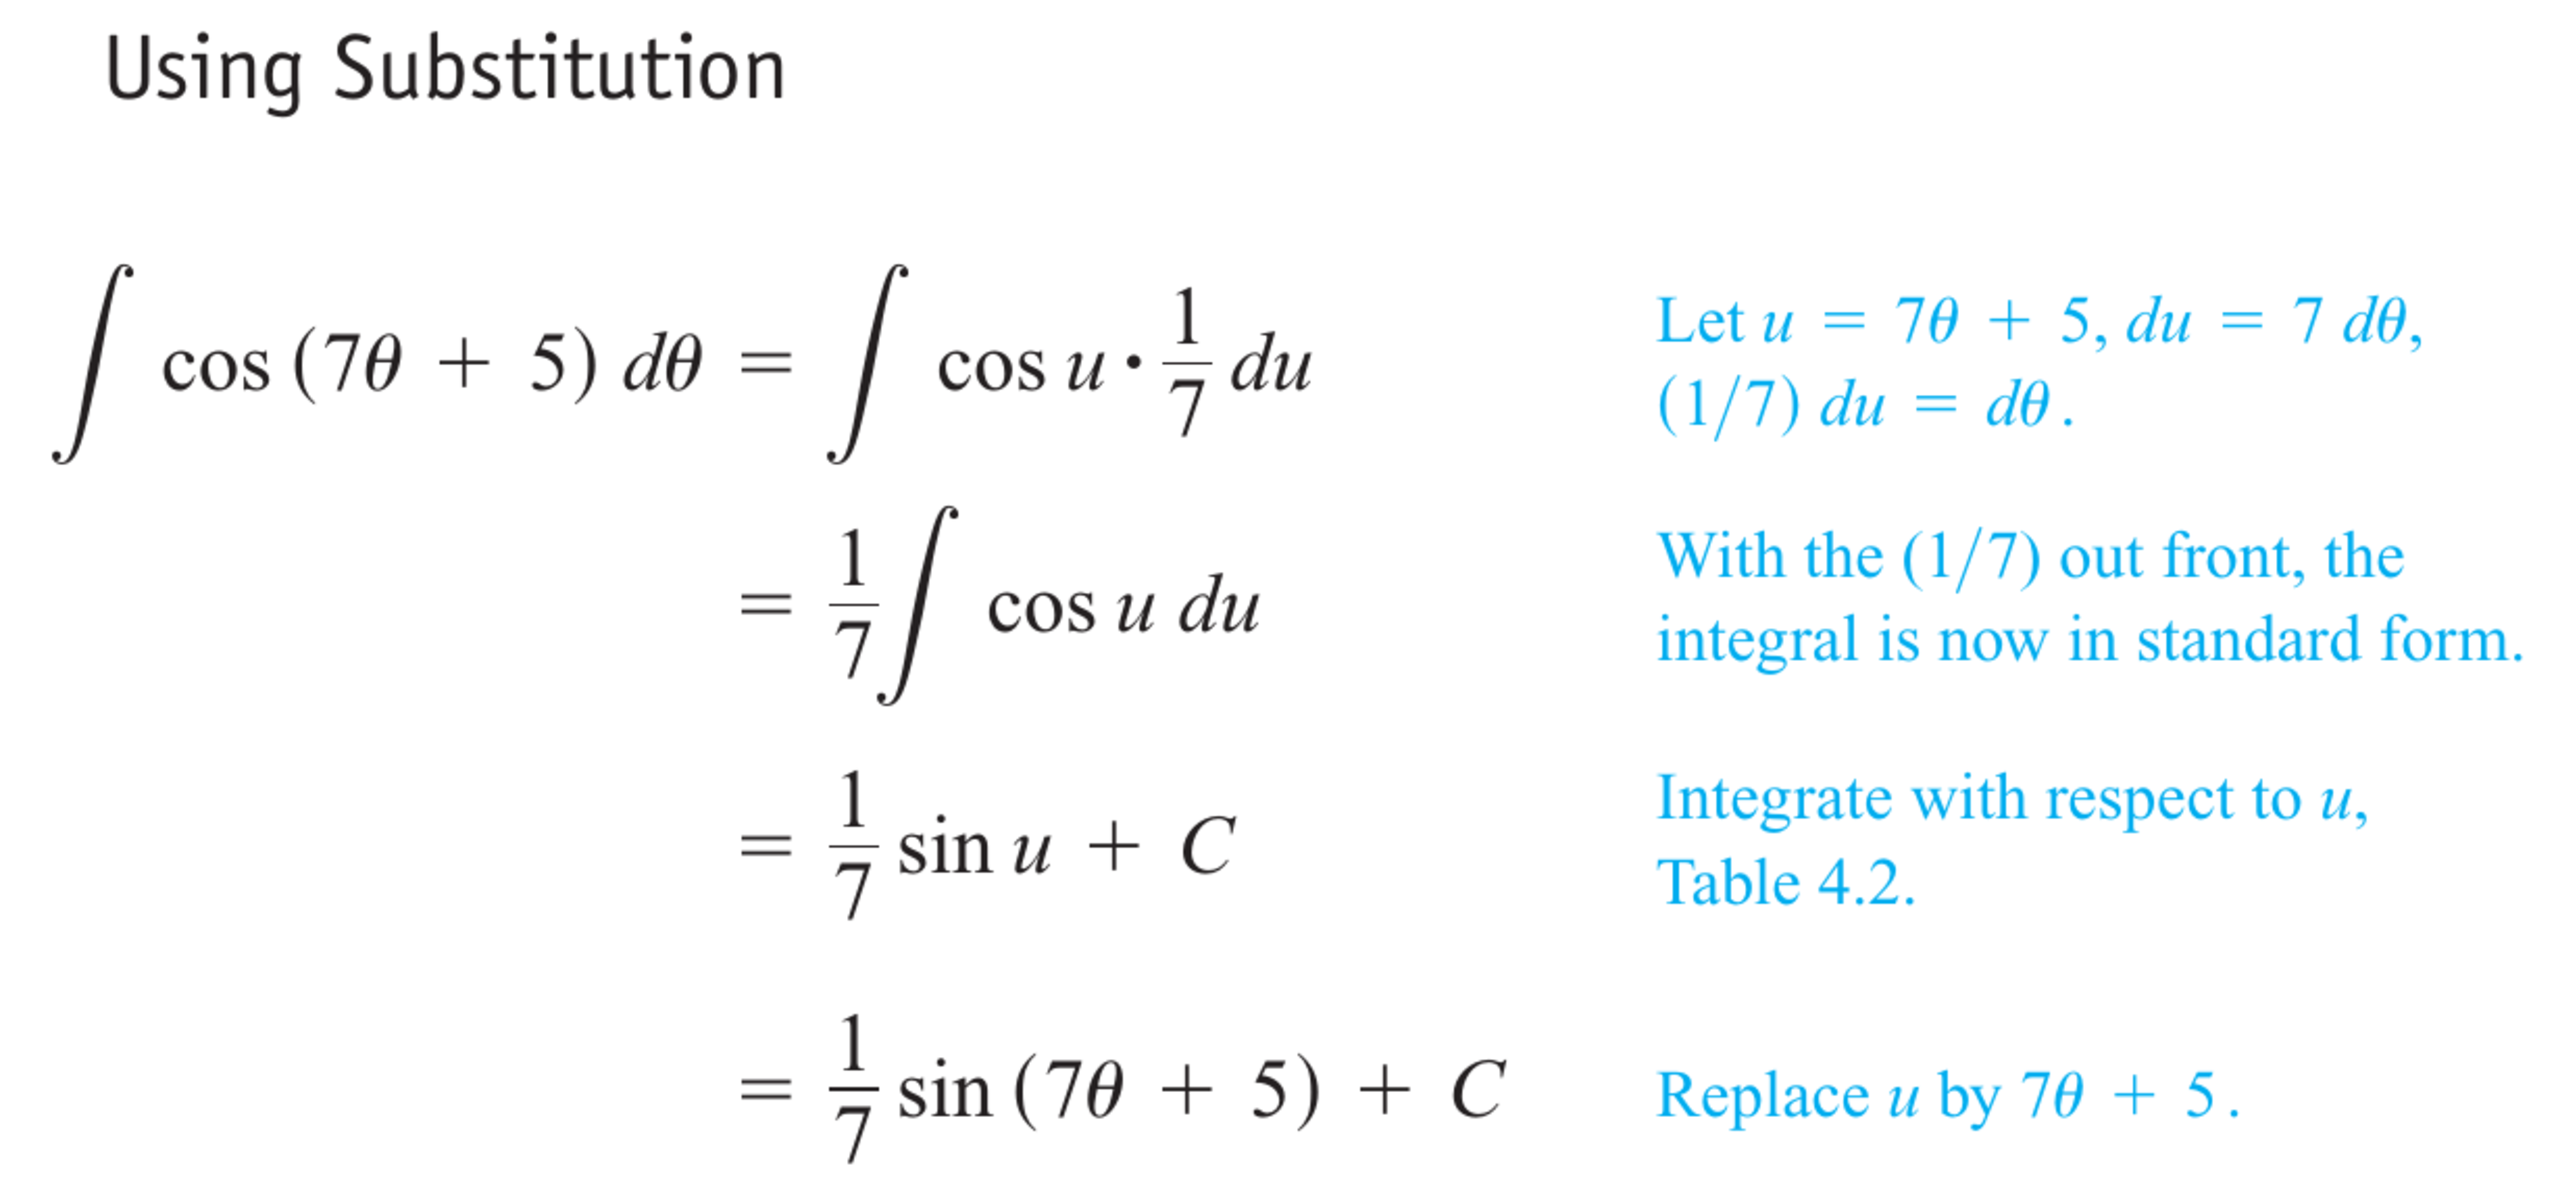
\includegraphics[width=9cm]{2021-2-C2/thomas11-p370-example-3.pdf}$$


Eu comecei a aprender um desses ``programas que entendem
demonstrações'' em 2021 -- o Lean:

\ssk

{\footnotesize

\url{https://www.ma.imperial.ac.uk/~buzzard/xena/}

}

\ssk

Ele é considerado muito mais fácil de usar que os ``proof assistants''
anteriores a ele mas ele ainda é bem difícil. Existem tutoriais pra
ele nos quais os usuários têm que demonstrar na linguagem do Lean
montes de exercícios de Matemática Discreta e Cálculo 1, mas acho que
ainda falta bastante pra alunos de primeiro período conseguirem
resolver os seus exercícios na linguagem do Lean.

}\anothercol{

Eu vou fazer algumas referências ao Lean no curso, meio como
curiosidade e meio por conta de uma coisa cuja explicação é meio
longa. Lá vai.

\bsk

Uma das coisas que me dá mais ódio é ter que lidar com alunos que
escrevem um monte de contas totalmente sem pé nem cabeça nas provas e
depois juram que ``tava tudo certo, caramba'' e que eu só dei nota
baixa pra eles porque eu tava de marcação com eles. E tem uma coisa
que me dá tipo 1/100 desse ódio, que é lidar com alunos que fazem
demonstrações nos quais eles pulam montes de passos e juram que tudo
que eles fizeram ``é óbvio''.

\msk

Neste curso nós vamos ver as definições \ColorRed{precisas} de {\sl
  alguns tipos} de ``passos óbvios'' que aparecem em demonstrações e
contas que são comuns de Cálculo 2. A maioria das demonstrações que
nós vamos ver são por sequências de igualdades, e vão ter este
formato:

$$\begin{array}{rcll}
    \Expr &=& \Expr & \Just \\
          &=& \Expr & \Just \\
          &=& \Expr & \Just \\
          &=& \Expr & \Just \\
  \end{array}
$$

A operação de substituição que eu vou explicar nos próximos slides vai
servir pra \ColorRed{ZILHÕES} de coisas durante o curso -- entre elas
pra gente entender quais passos da forma abaixo são ``óbvios'':
%
$$\begin{array}{rcll}
    \Expr &=& \Expr & \Just \\
  \end{array}
$$


\bsk
\bsk
\bsk
\bsk
\bsk

Obs: eu copiei o texto acima daqui: \Ca{2dT8}

Falta revisá-lo!

}}

% (find-thomas11-1page (+ 58 344) "Notation and existence of the definite integral")
% (find-thomas11-1page (+ 61 370) "Example 2")
% (find-thomas11-1page (+ 61 371) "Example 3")

% https://en.wikipedia.org/wiki/Lambda_calculus#Substitution



\newpage


%  ____        _       ____  
% | __ )  ___ | |__   |___ \ 
% |  _ \ / _ \| '_ \    __) |
% | |_) | (_) | |_) |  / __/ 
% |____/ \___/|_.__/  |_____|
%                            
% «atirei»  (to ".atirei")
% (c2m231introp 8 "atirei")
% (c2m231introa   "atirei")
% (c2m222srp 3 "atirei")
% (c2m222sra   "atirei")

{\bf Atirei o Pau no Gato: seja como o Bob}

\scalebox{0.7}{\def\colwidth{8cm}\firstcol{

Imagina que você está fazendo aula de flauta doce junto com o Alex e o
Bob, e na prova vocês vão ter que tocar Atirei o Pau no Gato.

O Alex demora um tempão pra encontrar cada nota, e ele leva meia hora
pra tocar a música toda.

O Bob toca a música toda certinha em menos de 30 segundos.

Quando saem as notas o Alex tirou uma nota baixa e o Bob tirou 10.

Aí o Alex vai chorar pontos e diz ``{\sl pôxa, profe, eu me esforcei
  muito!}''

\bsk

Quando o Bob tocou Atirei o Pau no Gato ele fez a música {\sl parecer
  fácil}. O esforço dele {\sl ficou invisível}.

\msk

\standout{Seja como o Bob!}

%\bsk
%\bsk


}\anothercol{

  O curso vai ter uma parte em que você vai ter que aprender a
  desenhar figuras com dezenas de retângulos e trapézios {\sl em
    poucos segundos} -- como o Bob tocando Atirei o pau no gato.

\ssk

  Se você for como o Alex, e levar mais de meia hora pra desenhar cada
  figura dessas, eu vou considerar que você não aprendeu os padrões
  que essas figuras seguem -- e você não aprendeu a coisa mais
  importante.

\ssk

  Logo depois dessa parte do curso vai vir uma parte em que você vai
  ter que visualizar mentalmente (limites de) figuras feitas de
  infinitos retângulos e trapézios, e desenhar essas figuras. Se você
  for como o Alex você vai levar tempo \ColorRed{infinito} pra
  desenhar cada uma dessas figuras; \ColorRed{se você for como o Bob
    você vai levar segundos}.

\msk

\standout{Seja como o Bob!}


}}


\newpage

%  ____        _       _____ 
% | __ )  ___ | |__   |___ / 
% |  _ \ / _ \| '_ \    |_ \ 
% | |_) | (_) | |_) |  ___) |
% |____/ \___/|_.__/  |____/ 
%                            
% «imagens-de-intervalos»  (to ".imagens-de-intervalos")
% (c2m231introp 11 "imagens-de-intervalos")
% (c2m231introa    "imagens-de-intervalos")
% (c2m222srp 13 "imagens-de-intervalos")
% (c2m222sra    "imagens-de-intervalos")

{\bf Imagens de intervalos}

\scalebox{0.5}{\def\colwidth{11.2cm}\firstcol{

Veja as páginas 5 e 7 daqui:

\ssk

{\footnotesize

% (c2m221somas3p 5 "imagens-figuras")
% (c2m221somas3a   "imagens-figuras")
%    http://angg.twu.net/LATEX/2022-1-C2-somas-3.pdf#page=5
\url{http://angg.twu.net/LATEX/2022-1-C2-somas-3.pdf\#page=5}

}

\msk

Digamos que na sua turma de Cálculo 2 tem dois Alexes diferentes, um
Bob, um Carlos e um Daniel, e todo mundo tá tentando resolver um
exercício que é o seguinte: ``seja $f$ a função da página 5 do link
acima. Calcule $f([1,3])$''.

Todo mundo reconhece que o intervalo $[1,3]$ é um conjunto com
infinitos pontos, e cada pessoa tenta resolver esse exercício de um
jeito diferente.

\msk

O Alex 1 decide começar listando todos os pontos do intervalo $[1,3]$.
Ele vai primeiro obter uma lista de pontos que ele vai escrever nesse
formato aqui,
%
$$\{x_1,x_2,x_3,x_4,\ldots\}
$$

e depois ele vai simplificar esse conjunto daqui,
%
$$\{f(x_1),f(x_2),f(x_3),f(x_4),\ldots\}
$$

transformando ele numa lista de números, pondo os números dessa lista
em ordem e deletando as repetições... \ColorRed{só que como o conjunto
  $\{x_1,x_2,x_3,x_4,\ldots\}$ é infinito ele nunca consegue terminar
  o primeiro passo.}

\msk

O Alex 2 decide que ele vai pegar uma sequência de conjuntos finitos
cada vez maiores, e ``cada vez mais parecidos'' com o conjunto
$[1,3]$. Ele escolhe essa sequência aqui...

}\anothercol{

%
$$\begin{array}{rcl}
  A_1 &=& \{1,3\}, \\
  A_2 &=& \{1,2,3\}, \\
  A_3 &=& \{1,1.5,2,2.5,3\}, \\
  A_4 &=& \{1,1.25,1.5,1.75,2,2.25,2.5,2.75,3\}, \ldots \\
  \end{array}
$$

Ele calcula $f(A_1)$, $f(A_2)$, $f(A_3)$, $f(A_4)$ pelo gráfico usando
o ``jeito esperto'' -- como nas figuras da página 5 do link -- e ele
deduz, \ColorRed{por um argumento informal e olhométrico}, que
$f([1,3])$ \ColorRed{deve ser} o intervalo $[3,4]$.

\msk

O Bob faz algo parecido como o Alex 2, mas ele encontra um modo de
``levantar'' todo o intervalo $[1,3]$ pro gráfico da função $y=f(x)$
de uma vez só, e de depois ``projetar'' pro eixo $y$ esse ``intervalo
levantado''. Ele obtém uma figura bem parecida com a última figura da
página 5 do link, e ele descobre -- \ColorRed{também meio no
  olhômetro} -- que $f([1,3]) = [3,4]$.

\msk

O Carlos vê que \ColorRed{é óbvio que}
$f([1,3]) = [f(1),f(3)] = \{3,3\} = \{3\}$, e \ColorRed{portanto} a
imagem do intervalo $[1,3]$ pela função $f$ é um conjunto com um ponto
só. $\frown$

\msk

O Daniel resolve que tudo isso é informal demais pra ele, e que ele
precisa aprender um modo 100\% preciso e formal de calcular $f([1,3])$
sem o gráfico. Ele descobre que vai ter que estudar uma coisa chamada
``Análise Matemática'', baixa o ``{\sl Elementary Analysis: The Theory
  of Calculus}'' do Kenneth Ross, começa a estudar por ele e aprende
coisa incríveis -- \ColorRed{mas ele leva um ano nisso}.

\msk

\standout{Seja como o Bob!}

}}


\newpage

%  ____            _                               
% |  _ \ ___  _ __| |_ _   _  __ _ _   _  ___  ___ 
% | |_) / _ \| '__| __| | | |/ _` | | | |/ _ \/ __|
% |  __/ (_) | |  | |_| |_| | (_| | |_| |  __/\__ \
% |_|   \___/|_|   \__|\__,_|\__, |\__,_|\___||___/
%                            |___/                 
% «sobre-portugues»  (to ".sobre-portugues")
% (c2m231introp 10 "sobre-portugues")
% (c2m231introa    "sobre-portugues")

{\bf Sobre Português}

\def\eqq{\overset{?}{=}}

\scalebox{0.52}{\def\colwidth{10.5cm}\firstcol{

Muita gente aprende no Ensino Médio e nas matérias de primeiro período
que ``entender uma fórmula'' quer dizer 1) traduzí-la pra português e
2) generalizá-la. Então é BEM comum uma pessoa ficar em dúvida se
pode fazer um passo como este aqui numa conta,
%
$$\sqrt{42^2 + 99^2} = 42 + 99$$

e aí a pessoa me perguntar isso aqui:

\begin{quote}
  Professor, a raiz quadrada de um número ao quadrado mais outro número
  ao quadrado é o número mais o outro número?
\end{quote}

É bem mais fácil discutir essa dúvida se a pessoa me fizer essa
pergunta em notação matemática, ou me mostrando a igualdade acima e
perguntando ``isso aqui é verdade?'', ou me mostrando isso aqui,
%
$$\sqrt{42^2 + 99^2} \eqq 42 + 99$$

que é bem mais bacana porque o `$\eqq$' deixa super claro que isso é
uma igualdade que a pessoa não sabe se é verdade...

}\anothercol{

  Se a pessoa me pergunta se isso aqui é verdade,
  %
  $$\sqrt{42^2 + 99^2} = 42 + 99 \qquad(*)$$
  %
  eu posso mostrar pra ela essa outra igualdade aqui -- note que eu
  estou dando nomes como $(*)$ e $(**)$ pras igualdades --
  %
  $$\sqrt{x^2 + y^2} = x + y \qquad({*}{*})$$
  %
  e aí eu pergunto ``você quer saber se a $({*}{*})$ é algo que vale
  sempre, né?'', e aí a pessoa responde ``É! É isso!'', e aí eu
  consigo responder: se a $(**)$ valer sempre ela também vai valer no
  caso em que $x=3$ e $y=4$. Quando $x=3$ e $y=4$ a $(**)$ vira isso
  aqui:
  %
  $$\sqrt{3^2 + 4^2} = 3 + 4 \qquad({*}{*}{*})$$
  %
  e aí temos:
  $$\def\und#1#2{\underbrace{#1}_{#2}}
    \def\setdepthto#1#2{\setbox1\hbox{$#2$}%
                        \dp1=#1%
                        \box1}
    \def\X   {\setdepthto{2pt}{x}}
    \def\Y   {\setdepthto{2pt}{y}}
    \def\X   {\mathstrut x}
    \def\Y   {\mathstrut y}
    \def\XSQ {\und{{{\und{\X}{3}}^2}}{9}}
    \def\YSQ {\und{{{\und{\Y}{4}}^2}}{16}}
    \def\XYSQ{\und{\XSQ+\YSQ}{25} \mathstrut}
    \def\LIN {\setdepthto{2pt}{\XYSQ}}
    \def\LOUT{\und{\setdepthto{50pt}{\sqrt{\LIN}}}{5}}
    \def\ROUT{\und{3+4 \mathstrut}{7}}
    \und{\LOUT \;=\; \ROUT}{\False}
  $$

  Ou seja, a igualdade $({*}{*}{*})$ é falsa, e portanto a $({*}{*})$
  não vale sempre.


%generalizar e especializar

%pronúncia - quase sempre tem, e nos ajuda

}}

\newpage


%  ____            _                                 ____  
% |  _ \ ___  _ __| |_ _   _  __ _ _   _  ___  ___  |___ \ 
% | |_) / _ \| '__| __| | | |/ _` | | | |/ _ \/ __|   __) |
% |  __/ (_) | |  | |_| |_| | (_| | |_| |  __/\__ \  / __/ 
% |_|   \___/|_|   \__|\__,_|\__, |\__,_|\___||___/ |_____|
%                            |___/                         
%
% «sobre-portugues-2»  (to ".sobre-portugues-2")
% (c2m231introp 11 "sobre-portugues-2")
% (c2m231introa    "sobre-portugues-2")

{\bf Sobre Português (e generalizar)}

\scalebox{0.6}{\def\colwidth{9cm}\firstcol{

    Repara que eu não descobri se a igualdade $(*)$ era verdade ou
    não... eu convenci a pessoa a discutir a igualdade $(**)$ ao invés
    disso, porque eu ``adivinhei'' que na verdade o que a pessoa
    queria saber era se a $(**)$ era verdade ou não. Além disso eu
    desmontei a pergunta original da pessoa -- aliás, a pergunta sobre
    a $(**)$ -- em várias perguntas menores.

    \msk

    Até alguns semestres atrás eu achava que todo chegava na
    universidade sabendo ``generalizar'' e ``particularizar'' (ou:
    ``especializar'') bastante bem... eu achava que as pessoas
    aprendiam isso assim que aprendiam a fazer ``contas com letras''
    no Ensino Médio.

    \msk

    Vocês provavelmente vão ouvir histórias sobre como os meus cursos
    de Cálculo em 2022.1 -- logo depois do fim da quarentena -- foram
    os piores cursos {\sl do universo}. Uma boa parte da razão pra
    isso foi que eu fiquei tentando encontrar modos de ensinar as
    pessoas a generalizarem e particularizarem, e fui descobrindo que
    essas coisas são muito mais difíceis de aprender e de ensinar do
    que eu pensava.

}\anothercol{

  A pessoa do slide anterior achava que só podia fazer uma pergunta se
  ela 1) generalizasse a pergunta dela, e 2) traduzisse a pergunta
  dela pra Português. Acho que ela achava que tinha que tratar essas
  duas coisas como se fossem fáceis e óbvias -- {\sl mas não são}, e
  eu recomendo que a gente trate particularização/especialização como
  algo difícil em que é muito comum as pessoas terem dúvidas muito
  importantes que vale a pena discutir, ``encontrar a generalização
  certa'' como algo BEM difícil e BEM importante que a gente vai
  treinar explicitamente em vários exercícios difíceis e importantes
  do curso, e a gente vai ver que ``traduzir pra português'' é uma
  ferramenta bem menos útil do que parece. Quase todas as expressões
  matemáticas que a gente vai ver têm uma pronúncia padrão, mas vai
  ser bem comum a ``tradução pra português'' não nos ajudar nada, ou
  até nos atrapalhar, porque a gente vai ter que entender algumas
  palavras e expressões ``como matemáticos'' e não no sentido usual
  delas...

  \msk

  (Veja o próximo slide!)

}}




\newpage

%  ____                                
% | __ )  __ _ _ __   __ _ _ __   __ _ 
% |  _ \ / _` | '_ \ / _` | '_ \ / _` |
% | |_) | (_| | | | | (_| | | | | (_| |
% |____/ \__,_|_| |_|\__,_|_| |_|\__,_|
%                                      
% «banana»  (to ".banana")
% (c2m231introp 12 "banana")
% (c2m231introa    "banana")

{\bf Banana}

\scalebox{0.5}{\def\colwidth{10.5cm}\firstcol{

Considere as quatro perguntas abaixo:

\begin{enumerate}

\item Qual é o resultado de substituir na palavra ``banana'' todas as
letras `a' por `w'?

\item Qual é o resultado de substituir na palavra ``banana'' todas as
letras `o' por `u'?

\item Qual é o resultado de substituir na palavra ``banana'' todas as
letras `A' por `W'?

\item Qual é o resultado de substituir na palavra ``blitiri'' todas as
letras `2' por `3'?

\end{enumerate}

O resultado da 1 é bem fácil: ``bwnwnw'', mas a maioria das pessoas
fica em dúvida nos outros itens... muitas pessoas respondem coisas
como ``não dá pra fazer o 2 porque ``banana'' não tem `o'\,'', ``não
sei se o 3 tem que dar ``bWnWnW'' ou ``bwnwnw''\,'', ou ``não dá pra
fazer o 4 porque ``blitiri'' não é uma palavra e `2' e `3'\,'' não são
letras''...

\msk

Neste curso, e em todos os cursos de matemática que vão vir depois
dele, \ColorRed{você vai ter que aprender a interpretar certas
  definições ``como matemático'':} você vai ter que descobrir a
interpretação mais simples possível que faça sentido, e essa idéia de
``mais simples possível'' vai ser bem \ColorRed{parecida} com {\sl
  fazer o programa mais simples possível que obedeça uma certa
  especificação}...

}\anothercol{

  Por exemplo:

  \ssk

  o programa que responde ``banana'' no item 2 é bem mais simples do
  que o programa que primeiro testa se a palavra original tem alguma
  letra `o', e dá erro se não tem;

  \ssk

  o programa que responde ``banana'' no item 3 -- porque ele considera
  que `a' e `A' são letras completamente diferentes, e ``banana'' não
  tem `A' -- é muito mais simples do que os programas que consideram
  que `a' e `A' são ``letras parecidas'';

  \ssk

  o programa que responde ``blitiri'' no item 4 é muito mais simples
  do que os programas que testam se a palavra original é uma palavra
  válida e se as duas letras dadas são caracteres considerados como
  ``letras''.

  \bsk
  \bsk
  \bsk
  \bsk
  \bsk
  \bsk

  Links:

  Sobre áreas negativas e retângulos degenerados:

  \Ca{2cT185}, \Ca{2cT185}

  \Ca{2fT63}, \Ca{2fT64}
  
  \ssk

  \Ca{2gT20} Contexto / Sabemos que $2=3$. Então...

  \Ca{2gT38} O macaco substituidor: banana

}}



\newpage

%  _   _                                 _           _               __ 
% | | | |_ __   _____  ___ __   ___  ___| |_ ___  __| |   ___  ___  / _|
% | | | | '_ \ / _ \ \/ / '_ \ / _ \/ __| __/ _ \/ _` |  / _ \/ _ \| |_ 
% | |_| | | | |  __/>  <| |_) |  __/ (__| ||  __/ (_| | |  __/ (_) |  _|
%  \___/|_| |_|\___/_/\_\ .__/ \___|\___|\__\___|\__,_|  \___|\___/|_|  
%                       |_|                                             
% «unexpected-eof»  (to ".unexpected-eof")
% (c2m231introp 13 "unexpected-eof")
% (c2m231introa    "unexpected-eof")

{\bf Unexpected end of input}

\scalebox{0.6}{\def\colwidth{9cm}\firstcol{

Uma coisa que me desespera{\sl va} bastante era quando um aluno me
mostrava algo como isso aqui,
%
$$\ddx(α(x)·β(x)) = α'(x)\;·$$

e me perguntava ``isso aqui tá certo?'', ou: ``é isso?''...

Aqui a pergunta mais precisa seria ``esse início tá certo?'', ou
``como é que eu continuo?''... eu aqui eu poderia responder ou
``não!'' ou isto,
%
$$\ddx(α(x)·β(x)) = α'(x)·β(x) + α(x)·β'(x)$$

só que a resposta que funciona melhor {\sl didaticamente} é a
seguinte:
%
$$\ddx(α(x)·β(x)) = α'(x)\;· \qquad (*)$$

não é nem mesmo uma
expressão válida, e um compilador que for analisar essa expressão vai
abortar no meio do parsing e dizer ``Unexpected end of input'', que é
um tipo específico de erro de sintaxe...

}\anothercol{

  O melhor modo de discutir a dúvida da pessoa que perguntou o ``isso
  aqui tá certo?'' é ir consertando com ela a expressão dela passo a
  passo, e -- \ColorRed{\bf JURO} -- o melhor modo de fazer isso é
  primeiro transformar a expressão dela em uma expressão que compile,
  como essa aqui:
%
$$\ddx(α(x)·β(x)) = α'(x)·42 \qquad (**)$$

que é uma igualdade -- no sentido de que tem uma representação em
árvore com o `=' no topo -- é aí a gente pode começar a discutir
coisas como:

\begin{itemize}

\item a igualdade $(**)$ é verdadeira para todas as funções $α(x)$ e
  $β(x)$?

\item a igualdade $(**)$ é um caso particular da regra do produto?

\end{itemize}



}}


\newpage


%  _____            _ _                     _                 ____  ____  _____ 
% | ____|_  ___ __ | (_) ___ __ _ _ __   __| | ___     ___   |  _ \|  _ \|  ___|
% |  _| \ \/ / '_ \| | |/ __/ _` | '_ \ / _` |/ _ \   / _ \  | |_) | | | | |_   
% | |___ >  <| |_) | | | (_| (_| | | | | (_| | (_) | | (_) | |  __/| |_| |  _|  
% |_____/_/\_\ .__/|_|_|\___\__,_|_| |_|\__,_|\___/   \___/  |_|   |____/|_|    
%            |_|                                                                
%
% «explicando-o-PDF»  (to ".explicando-o-PDF")
% (c2m231introp 14 "explicando-o-PDF")
% (c2m231introa    "explicando-o-PDF")

{\bf ``Faz um vídeo explicando o PDF''}

\scalebox{0.6}{\def\colwidth{9.5cm}\firstcol{

    Em 2021 em fiz um vídeo -- que ficou bem bom -- pra responder os
    alunos que estavam dizendo ``professor, faz um vídeo explicando o
    PDF'', e em 2023 eu legendei esse vídeo. Dá pra acessar as
    legendas e o vídeo nos links abaixo,

% (find-angg ".emacs.videos" "c2m211somas1d")

\ssk

{\footnotesize

%              (find-TH "2021-1-C2-somas-1-dicas")
%  (find-angg "SUBTITLES/2021-1-C2-somas-1-dicas.lua")
% file:///home/edrx/TH/L/2021-1-C2-somas-1-dicas.html
\url{http://anggtwu.net/2021-1-C2-somas-1-dicas.html}

}

\ssk

e o trecho mais importante das legendas é esse aqui:

\bsk

Então, cada PDF tem vários exercícios e muitas dezenas de idéias. Se
vocês disserem só ``faz um vídeo explicando o PDF'' eu vou fazer um
vídeo de 5 minutos explicando tudo de um PDF por alto porque eu não
sei direito onde estão as dúvidas de vocês... mas vocês fizerem
perguntas mais específicas aí eu consigo fazer vídeos bem mais
detalhado sobre aquelas perguntas ou sobre aqueles exercícios...
gente, vocês não estão discutindo para descobrir como resolver os
problemas? O próximo passo, já que vocês estão empacados, é vocês
passarem a discutir pra encontrar a boas perguntas pra fazer... aqui
tem um outro trecho que eu não copiei, e deixa eu só ler isso aqui em
voz alta também...


}\anothercol{

gente, a matéria de matemática fica cada vez mais
difícil à medida que as matérias ficam mais avançadas, e passa a ser
comum ter trechos uma linha ou de um parágrafo nos livros-texto que
vocês vão passar muitas horas tentando decifrar aquilo. Isso vai
acontecer O TEMPO TODO... praticamente toda aula, toda página, todo
vídeo vai acontecer isso, até o a última matéria de matemática na vida
de vocês, então a questão é: como é que vocês podem fazer para não
ficarem perdidos com isso, para não ficarem paralisados... voltando
pro que eu escrevi aqui, o meu objetivo aqui é fazer vocês aprenderem
se virar com isso, e a técnica para isso e vocês aprenderem a escrever
as hipóteses de vocês e aprenderem a fazer perguntas. A maioria das
perguntas vocês vão conseguir responder sozinhos, algumas vocês vão
conseguir descobrir a resposta conversando com amigos -- faltou um ``s''
aqui... -- que também não sabiam a resposta, que vão descobrir junto
com vocês, e umas poucas vocês vão empacar mesmo e não vão conseguir
resolver sozinhos. Me mandem as dúvidas de vocês!

}}


\newpage

%     _                  _         _   _      _       
%    / \   _ __   __ _  | |    ___| |_(_) ___(_) __ _ 
%   / _ \ | '_ \ / _` | | |   / _ \ __| |/ __| |/ _` |
%  / ___ \| | | | (_| | | |__|  __/ |_| | (__| | (_| |
% /_/   \_\_| |_|\__,_| |_____\___|\__|_|\___|_|\__,_|
%                                                     
% «ana-leticia»  (to ".ana-leticia")
% (c2m231introp 15 "ana-leticia")
% (c2m231introa    "ana-leticia")

{\bf Um post da Ana Leticia de Fiori}


\scalebox{0.47}{\def\colwidth{11.5cm}\firstcol{

Em 19/fev/2023 a Ana Letícia de Fiori

postou
\href{https://www.facebook.com/ana.fiori.353/posts/pfbid033q2U4dEPxjGgDG69R3NZevU5phGmtCS6HZZ9SYh7EVMZuNdisw2cFx3PimB5ecL9l}{isso
  aqui} no Facebook:

% https://www.facebook.com/ana.fiori.353/posts/pfbid033q2U4dEPxjGgDG69R3NZevU5phGmtCS6HZZ9SYh7EVMZuNdisw2cFx3PimB5ecL9l

\msk

{\bf AL:} Um fenômeno curioso que tenho observado entre estudantes que
declaram ter ``travas de escrita'', ficarem ``empacados'' ao
desenvolver trabalhos de conclusão de disciplinas ou de curso.
Frequentemente, a alegação é de que o ``perfeccionismo'' faz com que
travem.

Eu tenho provocado, perguntado sobre quais são os gatilhos, quais os
momentos em que eles sentem que o bloqueio vem. Uma resposta é o
confronto com o material coletado, sejam os dados sejam as referências
levantadas. Materiais com os quais eles não conseguem lidar, no
sentido radical da palavra lida. Não sabem trabalhar com as
referências e com os dados. Porque não estão acostumados a ler.

Um dos efeitos disso são trabalhos bastante declaratórios, que clamam
ter feito ``revisões bibliográficas'', ``levantamentos'', ``análises
de discurso'', etc. que, na verdade, jamais ocorreram. Ao finalmente
escrever, despreza-se o que consta na literatura e se escreve de
cabeça, com alguma citação aqui ou acolá utilizada como argumento de
autoridade. Claro que o texto sai confuso, raso, impreciso.

Passa longe de um problema de perfeccionismo. Mas é assim que se
mascara a falta de perícia no ofício acadêmico.

E, recentemente, numa reunião entre pares, ouvi dizerem que para
evitar os eternos problemas de plágio e os novos problemas dos
softwares de IA, vão só realizar atividades orais e de escrita em sala
de aula. Isso me apavora, porque o tempo de maturação de um trabalho
acadêmico não é o tempo da sala de aula. E vai ser mais uma instância
a sumir da experiência desses estudantes.

\msk

}\anothercol{

{\bf E:} Nossa, eu tou exatamente tentando escrever sobre um outro
tipo de "perfeccionismo" que alguns dos meus estudantes têm e que eu
ainda não tenho um modo muito bom de lidar com isso...

São estudantes que assim que vêem que algo que eles escreveram está
errado eles ou apagam ou jogam foram. Eu até tenho um monte de
material - e slogans - sobre como o modo mais rápido de aprender
assuntos difíceis de matemática é você escrever "hipótese" ou
"rascunho" antes das partes que você não tem certeza e NÃO APAGAR
NADA, NUNCA -

...mas não adianta, eles entram em pânico quando vêem que algo que
eles escreveram não está perfeito - e aí eles não conseguem estudar...


\msk

{\bf AL:} Mas aí é que está, a que parâmetros de perfeição eles se
referem?

Esse comportamento de escrever e apagar tem a ver em parte com a
fantasia de que o texto se compõe de uma vez só. Tendem a pular as
etapas de estruturação de um roteiro, de rascunhos e revisões.

Quase como se o texto fosse psicografado. Eu costumo brincar com meus
alunos que ninguém é Chico Xavier da antropologia, eles riem, mas
teimam.

De novo, falta a dimensão do trabalho com o texto.

Perfeição, na fantasia dos alunos, é escrever sem esforço.

}}



\newpage

%  ____      _                                                    
% |  _ \ ___| |_ __ _ ___   _ __ _____   _____ _ __ ___  __ _ ___ 
% | |_) / _ \ __/ _` / __| | '__/ _ \ \ / / _ \ '__/ __|/ _` / __|
% |  _ <  __/ || (_| \__ \ | | |  __/\ V /  __/ |  \__ \ (_| \__ \
% |_| \_\___|\__\__,_|___/ |_|  \___| \_/ \___|_|  |___/\__,_|___/
%                                                                 
% «retas-reversas»  (to ".retas-reversas")
% (c2m231introp 16 "retas-reversas")
% (c2m231introa    "retas-reversas")
% https://math.stackexchange.com/questions/2353288/point-to-line-distance-in-3d-using-cross-product

{\bf Retas reversas}

\scalebox{0.55}{\def\colwidth{9.5cm}\firstcol{

    O Alex, o Bob e o Carlos fizeram GA juntos. Um dos últimos
    assuntos do curso era uma fórmula pra calcular a distância entre
    ``retas reversas'' -- é uma fórmula bem complicada, que tem um
    determinante e um produto cruzado -- e cada um deles estudou esse
    assunto de um modo diferente.

    \msk

    O Alex e o Carlos ``sabem'' que o objetivo de cada matéria de
    Matemática é fazer as pessoas aprenderem certos teoremas. Os dois
    decoraram a fórmula da distância entre retas reversas e tentaram
    aplicar ela na prova. O Alex conseguiu, mas a questão da prova
    tinha vários itens e em todos eles ela usava letras diferentes das
    da fórmula que ele tinha decorado, e aí ele levou MUITO tempo pra
    resolver um item, e não conseguiu fazer os outros... e o Carlos
    tinha decorado a fórmula errado, e aí num determinado ponto da
    questão ele precisava dividir um número negativo por um vetor, e
    ele não sabia como fazer isso.

    \msk

    {\sl Tanto o Alex quanto o Carlos esqueceram a fórmula logo depois
      da prova.}


}\anothercol{

  O Bob estudou essa parte da matéria de um outro jeito. Ao invés de
  pensar ``toda vez que eu precisar calcular a distância entre duas
  retas é só usar a fórmula'' ele considerou que tem muitos casos
  simples em que ele sabe calcular a distância entre as retas no
  olhômetro -- por exemplo, o caso em que uma das retas é paralela ao
  eixo $x$ e a outra é paralela ao eixo $y$. Ele foi aprendendo como
  lidar com vários casos um pouco menos simples que esse, e aprendeu
  como visualizar o que aquela fórmula complicadíssima ``quer dizer''
  -- ela calcula a altura de um certo paralelepípedo.

  \msk

  O Bob tratou essa fórmula como algo que generaliza vários casos
  ``simples'' em que ele consegue calcular a distância entre duas
  retas por outros métodos, e ele usou esses casos simples pra testar
  se a fórmula realmente dá o resultado que ele esperava.

  \msk

  Tanto o Alex quanto o Bob quanto o Carlos ``estudaram pelo livro'',
  mas existem vários modos de ``estudar pelo livro'' e o Bob usou
  modos que nem o Alex nem o Carlos conheciam.

  \msk

  {\sl Neste curso você vai aprender -- e treinar -- vários modos de
    ``estudar pelo livro'' que provavelmente vão ser totalmente novos
    pra você.}


}}


\newpage

% «contexto»  (to ".contexto")
% (c2m231introp 5 "contexto")
% (c2m231introa    "contexto")
% (c2m212introp 4 "contexto")
% (c2m212introa   "contexto")

{\bf Contexto}

\scalebox{0.6}{\def\colwidth{9cm}\firstcol{

    Quase todas as expressões matemáticas que usamos em C2
    \ColorRed{dependem do contexto}. Por exemplo, a interpretação
    \ColorRed{default} pra esta expressão aqui:
    % 
    $$f(x) = x-9 = 2$$

    é:
    % 
    $$\begin{tabular}{l}
        \ColorRed{Para toda} função $f:\R→\R$ \\
        e para todo $x∈\R$ temos: \\
        $f(x) = x-9 = 2$
      \end{tabular}
    $$

    Se você só escreve ``$f(x) = x-9 = 2$'' e mostra isso pro ``colega
    que seja seu amigo'' ele vai levar meia hora tentando adivinhar
    qual foi o contexto que você estava pensando mas não escreveu...
      
    ...e se ele descobrir em menos de, digamos, 50 tentativas, ele
    vai dizer ``ok, jóia, tá certo!''.

}\anothercol{

    O ``colega que seja menos seu amigo'' vai fazer menos tentativas,
    e os personagens ``o monitor'' e ``o professor'' da Dica 7 vão
    checar se o que você escreveu vai ser entendido corretamente por
    qualquer pessoa que saiba as convenções de como escrever
    matemática.

    \msk

    Lembre que \ColorRed{quase todo mundo} pára de ler um texto matemático
    quando vê uma besteira muito grande escrita nele. Imagine
    que um ``colega que seja menos seu amigo'' te mostra a
    solução dele pra um problema e te pergunta se está certa.
    A solução dele começa com:
    %
    $$\text{Sabemos que $2=3$. Então...}$$

    O que você faria?

    \bsk
    \bsk
    \bsk
    \bsk
    \bsk

    Dica: releia isto aqui:

    \Ca{Slogans27:07} até 32:45

}}





\newpage

%  _____                          _                    _     _           
% |  ___|__  _ __ _ __ ___  _   _| | __ _ ___    ___  | |__ (_)_ __  ___ 
% | |_ / _ \| '__| '_ ` _ \| | | | |/ _` / __|  / _ \ | '_ \| | '_ \/ __|
% |  _| (_) | |  | | | | | | |_| | | (_| \__ \ |  __/ | | | | | |_) \__ \
% |_|  \___/|_|  |_| |_| |_|\__,_|_|\__,_|___/  \___| |_| |_|_| .__/|___/
%                                                             |_|        
% «formulas-e-hipoteses»  (to ".formulas-e-hipoteses")
% (c2m231introp 17 "formulas-e-hipoteses")
% (c2m231introa    "formulas-e-hipoteses")

{\bf Fórmulas e hipóteses}

\scalebox{0.65}{\def\colwidth{8.5cm}\firstcol{

Dê uma olhada no Teorema 4 da seção 3.1 do Miranda:
\Ca{MirandaP80}. Ele diz isso aqui:

% \ssk
% 
% {\scriptsize
% 
% % (find-books "__analysis/__analysis.el" "miranda")
% % (find-books "__analysis/__analysis.el" "miranda" "3.4 Regras de Derivação")
% % (find-dmirandacalcpage 80 "3.4 Regras de Derivação")
% % (find-dmirandacalctext 80     "Regras de Derivação")
% %    http://hostel.ufabc.edu.br/~daniel.miranda/calculo/calculo.pdf#page=80
% \url{http://hostel.ufabc.edu.br/~daniel.miranda/calculo/calculo.pdf}
% 
% }

\begin{quote}

  Se $f$ e $g$ são funções diferenciáveis em $x = a$ então a função
  $f+g$ é diferenciável em $a$ e:
  %
  $$(f+g)'(a) = f(a) + g(a).$$

\end{quote}

Nós vamos considerar que esse {\sl teorema} pode ser decomposto em
duas partes: {\sl fórmula} e {\sl hipóteses}. A {\sl fórmula} dele é
esta aqui,
%
$$(f+g)'(a) = f(a) + g(a)$$

e em muitas situações nós vamos querer usar só as fórmulas de certos
teoremas e deixar pra verificar as hipóteses delas no final.


}\anothercol{


{\sl Obs: falta acrescentar muita coisa aqui... explicar o que são
  contas formais, mostrar que o Mathologer só faz contas formais no
  vídeo dele sobre o ``Calculus Made Easy'', mencionar que em Cálculo
  3 nós vamos usar o ``Calculus Made Easy'' e que todas as contas dele
  são formais, falar sobre a introdução do Martin Gardner pro CME e
  como ele explica que o conceito de ``função'' foi mudando...}


\bsk

Obs 2: tem um slide sobre contas formais aqui:

\Ca{2gT36} (p.4) O macaco e as contas formais

% {\footnotesize
% 
% % (c2m231macacop 4)
% %    http://anggtwu.net/LATEX/2023-1-C2-macaco.pdf#page=4
% \url{http://anggtwu.net/LATEX/2023-1-C2-macaco.pdf\#page=4}
% 
% }


}}




\newpage

% «aulas-expositivas»  (to ".aulas-expositivas")
% (c2m231introp 21 "aulas-expositivas")
% (c2m231introa    "aulas-expositivas")

{\bf Sobre aulas expositivas}

\scalebox{0.9}{\def\colwidth{12cm}\firstcol{

    % {\sl Sobre porque aulas puramente expositivas, ou aulas
    % principalmente expositivas, não funcionam.} Aqui vou ter que
    % usar duas expressões que são muito usadas em ensino de línguas
    % estrangeiras: ``vocabulário ativo'' e ``vocabulário passivo''.
    % Uma palavra está no seu ``vocabulário ativo'' se você consegue
    % usar ela quando você fala (ou escreve), e uma palavra está só no
    % seu ``vocabulário passivo'' quando você não usa ela mas você
    % entende ela quando alguém usa.

    Muitos alunos acreditam que se eles assistirem uma aula expositiva
    eles vão ser capazes de resolver na prova questões sobre o que
    eles aprenderam -- só que isso só passa a ser {\sl mais ou menos}
    verdade depois que a pessoa aprende {\sl muito bem} como estudar.

    \msk

    Muita coisa em matemática funciona como músculos. Os músculos
    mentais que você usa pra entender uma aula expositiva são bem
    diferentes dos músculos mentais que você usa pra resolver
    exercícios, e os músculos mentais que você exercita quando você
    relê uma explicação que você escreveu e procura jeitos de
    reescrevê-la de um modo mais claro são diferentes desses...

    \msk

    Leia isto aqui:

    \Ca{Visaud39:09} até 46:06

}\anothercol{
}}

\newpage

% «formal-vs-coloquial»  (to ".formal-vs-coloquial")
% (c2m231introp 22 "formal-vs-coloquial")
% (c2m231introa    "formal-vs-coloquial")

{\bf Formal vs.\ coloquial}

\scalebox{0.65}{\def\colwidth{8.2cm}\firstcol{

Lembre que um dos meus objetivos principais {\sl neste curso} é fazer
as pessoas aprenderem a escrever suas idéias matemáticas de um jeito
que seja claro e fácil de revisar, que elas gostem de reler depois
(dica 7b) e que os colegas gostem de ler (dicas 7c e 7d)...

\msk

Algumas pessoas acham que textos matemáticos têm que ser escritos numa
linguagem ``formal'' que seja a mais distante possível do português
coloquial; outras pessoas preferem escrever de um modo bem próximo do
coloquial. Por exemplo, o Jacir Venturi (\Ca{VenturiGA}), escreve num
Português pomposo que eu acho horrível, e o Felipe Acker
(\Ca{AckerGA1}) escreve de um modo bem próximo do coloquial que eu
gosto bastante. E até hoje eu só tive acesso a bem pouco material do
Reginaldo, mas eu tenho a impressão de que ele não gosta de usar
linguagem coloquial em matemática... eu falo um pouquinho sobre isso
neste trecho de um vídeo sobre didática: \Ca{Visaud59:49}.

}\anothercol{

% \vspace*{0.25cm}

Na parte do curso sobre somas de Riemann você vai aprender a lidar com
definições bem complicadas, e aos poucos -- um pouquinho neste curso,
e bastante nos seguintes -- você vai aprender a fazer as suas próprias
definições. E quando você souber fazer as suas próprias definições
você vai ver que dá pra ser totalmente preciso usando tanto português
coloquial quanto português pomposo...

\msk

...ah, e na parte final do curso, que é sobre equações diferenciais,
você vai (ter que) aprender a usar corretamente um monte de
``partículas'', como ``seja'', ``então'', ``temos'', ``isto é'',
``queremos'', ``sabemos que'', ``lembre que'', ``digamos que'' e
``vamos testar se''.

% \vspace*{0.25cm}
% 
% Note que a expressão ``linguagem formal'' tem vários sentidos
% diferentes -- o dos primeiros slides, 
% 
%  ``não-coloquial'' e ``preciso''. Dá pra gente ser preciso
% usando

}}




% % (c2m231introp 21 "vocabulario-ativo")
% % (c2m231introa    "vocabulario-ativo")
% %  (c2m222buracop 2 "macaco")
% %  (c2m222buracoa   "macaco")
% 
% 
% 
% 
% 
% \newpage
% 
% %  _   _ _             _                 
% % | | | (_)_ __   ___ | |_ ___  ___  ___ 
% % | |_| | | '_ \ / _ \| __/ _ \/ __|/ _ \
% % |  _  | | |_) | (_) | ||  __/\__ \  __/
% % |_| |_|_| .__/ \___/ \__\___||___/\___|
% %         |_|                            
% % «escreva-hipotese»  (to ".escreva-hipotese")
% % (c2m231introp 13 "escreva-hipotese")
% % (c2m231introa    "escreva-hipotese")
% % (find-angg "SUBTITLES/2021-1-C2-somas-1-dicas.lua" "legendas")
% 
% {\bf Não apague - escreva ``hipótese:''}
% 
% (...)
% 
%   Cumprimento superficial da matéria
% 
%   Os alunos acham que na hora da prova eles vão magicamente conseguir
%   fazer questões que ele não treinaram
% 
%   Toda dúvida é bem vinda. Dúvidas sobre assuntos ``antigos'' em
%   vários graus -- assuntos tratados algumas aulas antes, assuntos de
%   matérias anteriores, assuntos de ensino médio -- são todas
%   válidas... mas 
% 
% 
% \newpage
% 
% %  __  __             _ _             _       
% % |  \/  | ___  _ __ (_) |_ ___  _ __(_) __ _ 
% % | |\/| |/ _ \| '_ \| | __/ _ \| '__| |/ _` |
% % | |  | | (_) | | | | | || (_) | |  | | (_| |
% % |_|  |_|\___/|_| |_|_|\__\___/|_|  |_|\__,_|
% %                                             
% % «monitoria»  (to ".monitoria")
% % (c2m231introp 10 "monitoria")
% % (c2m231introa    "monitoria")
% 
% Cálculo 2 é uma disciplina na qual os alunos aprendiam técnicas
% importantíssimas à medida que faziam milhares de contas à mão; eles
% precisavam resolver muitas integrais e equações diferenciais sem
% errar, e precisavam descobrir praticamente sozinhos como não se perder
% e não errar nestas contas. Muitas das técnicas que eles aprendiam não
% estão explicadas explicitamente em livro nenhum.
% 
% Hoje em dia há bons programas de computação simbólica ("PCS"s) que
% rodam até em celulares e que resolvem em segundos as questões de
% Cálculo 2 que costumavam cair nas provas, e pessoas de vários lugares
% do Brasil estão discutindo como mudar a abordagem do curso de Cálculo
% 2 - sem mudar a ementa ou o programa - pra que os alunos aprendam as
% técnicas importantíssimas acima de outras formas. Os detalhes da minha
% abordagem atual estão aqui:
% \url{http://angg.twu.net/LATEX/2021-2-C2-tudo.pdf}. É fácil ver que, e
% como, os exercícios do "tudo.pdf" complementam os exercícios dos
% livros tradicionais: um dos focos do curso passa a ser aprender como
% manipular expressões algébricas de um jeito parecido com o que os PCSs
% fazem; outro, visualizar o que certas expressões "querem dizer", e
% outro, como definir precisamente o que é uma igualdade "óbvia". Alguns
% alunos estranham essa abordagem, e um monitor ajudaria muito.
% 
% 
% 
% 
% \newpage
% 
% {\bf Quando você crescer}
% 
% ...em equipe
% 
% contas fáceis de revisar
% 
% visualizar muita coisa de cabeça
% 
% erros conceituais graves
% 
% o computador vai fazer uma parte das contas
% 
% um resultado errado pode custar milhares de dinheiros








% EDOVSs
%  (c2m222p2p 5 "questao-1-gab")
%  (c2m222p2a   "questao-1-gab")

% Integração por partes:
%  (c2m222p1p 6 "questao-2-gab")
%  (c2m222p1a   "questao-2-gab")

% Nomes
% (c2m212p2p 8 "questao-3")
% (c2m212p2a   "questao-3")
% (c2m212p2p 9 "questao-3" "Daigoro")
% (c2m212p2a   "questao-3" "Daigoro")
% (find-arounds "Daigoro")

% Integrais impróprias
% (find-books "__analysis/__analysis.el" "miranda")
% (find-books "__analysis/__analysis.el" "miranda" "10 Integrais Impróprias")

% Igualdades com justificativas
% (c2m222buracop 4 "exercicio-1")
% (c2m222buracoa   "exercicio-1")

% A operação de substituição
% (c2m222buracop 5 "derivadas-formais")
% (c2m222buracoa   "derivadas-formais")
% (c2m221dvsp 3 "erros-sintaticos")
% (c2m221dvsa   "erros-sintaticos")

% (c2m221dfia "title")
% (c2m221dfia "title" "derivada" "da função inversa")
% (c2m221dfip 5 "demonstracao-complicada")
% (c2m221dfia   "demonstracao-complicada")

% Fórmulas, hipóteses, contas formais

% Uma prova bem antiga:
% (find-LATEX "2019-2-C2-P1.tex" "gabarito-maxima")


\GenericWarning{Success:}{Success!!!}  % Used by `M-x cv'

\end{document}


% Local Variables:
% coding: utf-8-unix
% ee-tla: "c2in"
% ee-tla: "c2m231intro"
% End:
